\documentclass[11pt]{article}
\usepackage[margin=1in]{geometry}
\usepackage{amsmath,booktabs,graphicx,siunitx,listings,longtable}
\usepackage[hidelinks]{hyperref}
\usepackage{bookmark}
\lstset{basicstyle=\ttfamily\scriptsize,breaklines=true,frame=single}
\title{Spice Analyzer Report: fan\_smc\_pin\_3}
\author{spice-analyzer}
\date{12 September 2026}
\begin{document}
\maketitle
\tableofcontents
\clearpage

\section{Analysis provenance}
\subsection{Agentic models}
\begin{center}
{\small
\begin{tabular}{@{}llllp{0.28\linewidth}@{}}
\toprule
Role & Host & Model & Scope & Notes \\
\midrule
Primary orchestrator & Cursor & Composer & ingest--report & skill spice-analyzer \\
\bottomrule
\end{tabular}}
\end{center}
\footnotesize Skill path: \texttt{.agents/skills/spice-analyzer}.
Toolchain: ngspice-45.2 (WSL); Python matplotlib plots; pdflatex.

\section{Circuit under test}
\subsection{Netlist and topology}
Source path: \texttt{Fan\_SMC\_Pin\_3}.
Subcircuit \texttt{fan\_smc\_pin\_3} pins: \texttt{gnda vdda vinn vinp vout}.
Topology: three-stage amplifier with Single Miller Compensation (SMC) and feedforward (FF) path.
\begin{itemize}
\item Stage 1 (\(g_{m1}\)): PMOS diff pair \texttt{xm8}/\texttt{xm9}, tail \texttt{xm4}, folded NMOS cascode \texttt{xm15}/\texttt{xm16}/\texttt{xm19}/\texttt{xm20}; first high-Z node \texttt{net050} (\(v_1\)).
\item Stage 2 (\(g_{m2}\)): PMOS \texttt{xm10} into diode \texttt{xm21}, mirrored by \texttt{xm22} to \texttt{net049} (\(v_2\)).
\item Stage 3 (\(g_{m3}\)): NMOS \texttt{xm23} to \texttt{VOUT}.
\item Feedforward (\(g_{mf}\)): PMOS \texttt{xm11} (gate=\texttt{net050}) to \texttt{VOUT}.
\item Compensation: \texttt{C0} between \texttt{net050} and \texttt{VOUT}; external \(C_L=\mathrm{CLOAD}\).
\end{itemize}
Seed sizing was placeholder \(W=L=1\,\mu\mathrm{m}\) at original \(V_{DD}=0.8\,\mathrm{V}\); fitted per backend (see Appendix).

\subsection{Device sizing table}
\begin{center}
{\small
\begin{tabular}{@{}lllll@{}}
\toprule
Role & Device & \(L\) & \(W\) & \(M\) \\
\midrule
gm1 PMOS & xm8/xm9 & 0.5 & 20 & 8 \\
gm2 PMOS & xm10 & 0.5 & 16 & 8 \\
gmf PMOS & xm11 & 0.5 & 10 & 16 \\
gm3 NMOS & xm23 & 0.5 & 20 & 16 \\
Bias CM PMOS & xm0.. & 1 & 4 & 8 \\
Bias CM NMOS & xm12.. & 0.5 & 4 & 4 \\
Load2 NMOS & xm21/22 & 0.5 & 8 & 4 \\
Passives & C0 / CL / Ib & n/a & 1\,pF / 10\,pF / 50\,\(\mu\)A & n/a \\
\bottomrule
\end{tabular}}
\end{center}
\footnotesize Table T0 --- sky130 fitted values (\texttt{option scale=1.0u}, \(W/L\) in \(\mu\mathrm{m}\)). Other backends retarget \(V_{DD}\) and \(W/L\) (see params).

\subsection{Backends, corners, MC scope}
Default pipeline: educational \texttt{cmos}, then open PDKs \texttt{sky130}, \texttt{ihp}, \texttt{gf180}.
Corners \texttt{tt/ff/ss} (or typical/ff/ss) on open PDKs.
MC: HARD-SKIP on all backends (Level-1 LOT agauss does not resample across trials; open-PDK mismatch MC not wired) --- see T8.

\section{Small-signal analysis (step-by-step)}
Primary hand numbers use \textbf{sky130} final OP after fit (\(V_{DD}=1.8\,\mathrm{V}\), \(V_{CM}=0.9\,\mathrm{V}\), \(C_c=1\,\mathrm{pF}\), \(C_L=10\,\mathrm{pF}\), \(I_b=50\,\mu\mathrm{A}\)).

\subsection{Step 0 --- Assumptions}
Saturation intended for signal FETs; OP shows \texttt{xm20} with large \(g_{ds}\) (triode/compressed cascode) --- noted in Rout trail.
Neglect device \(C_{gs}/C_{gd}\) vs \(C_c,C_L\) near GBW.
Hand \(g_m\) from OP; square-law shown for pedagogy then replaced by OP \(g_m\).

\subsection{Step 1 --- Bias currents}
Ideal ratios from netlist multipliers with \(I_b=50\,\mu\mathrm{A}\), \(M_p=8\):
\[
I_{\mathrm{tail}}=4 I_b=200\,\mu\mathrm{A},\quad
I_{\mathrm{leg}}\approx 100\,\mu\mathrm{A}\ \text{(balanced)}.
\]
OP shows unbalanced/starved input legs (\(I_{D,\mathrm{xm8}}=2.45\,\mu\mathrm{A}\), \(I_{D,\mathrm{xm9}}=5.07\,\mu\mathrm{A}\)) --- OP-assisted hand below.

\begin{center}
\begin{tabular}{lrrl}
\toprule
Device & Hand \(I_D\) & OP \(I_D\) & Note \\
\midrule
xm0 (Ib diode) & \(50\,\mu\mathrm{A}\) & OP-assist & \(I_b\) \\
xm4 (tail) & \(200\,\mu\mathrm{A}\) & OP-assist & \(4 I_b\) ideal \\
xm8 (gm1) & \(100\,\mu\mathrm{A}\) & \(2.45\,\mu\mathrm{A}\) & starved vs ideal \\
xm9 (gm1) & \(100\,\mu\mathrm{A}\) & \(5.07\,\mu\mathrm{A}\) & unbalanced \\
xm10 (gm2) & OP & \(50.9\,\mu\mathrm{A}\) & OP-assisted \\
xm23 (gm3) & OP & \(64.2\,\mu\mathrm{A}\) & OP-assisted \\
xm11 (gmf) & OP & \(64.2\,\mu\mathrm{A}\) & OP-assisted \\
\bottomrule
\end{tabular}
\end{center}
\footnotesize Table T1.

\subsection{Step 2 --- Transconductances}
Educational square-law (KP\(_p=100\,\mu\mathrm{A/V}^2\), KP\(_n=200\,\mu\mathrm{A/V}^2\); OP \(I_D\)) then replace by OP \(g_m\):
\begin{align*}
g_{m1,\mathrm{sq}}&=\sqrt{2\cdot KP_p\cdot(W/L)M\cdot I_{D8}}=\sqrt{2\cdot 100e-6\cdot(20/0.5)\cdot 8\cdot 2.454e-06}=3.963e-04\,\mathrm{S},\\
g_{m2,\mathrm{sq}}&=\sqrt{2\cdot KP_p\cdot(16/0.5)\cdot 8\cdot I_{D10}}=\sqrt{2\cdot 100e-6\cdot(16/0.5)\cdot 8\cdot 5.091e-05}=1.614e-03\,\mathrm{S},\\
g_{m3,\mathrm{sq}}&=\sqrt{2\cdot KP_n\cdot(20/0.5)\cdot 16\cdot I_{D23}}=\sqrt{2\cdot 200e-6\cdot(20/0.5)\cdot 16\cdot 6.419e-05}=4.054e-03\,\mathrm{S},\\
g_{mf,\mathrm{sq}}&=\sqrt{2\cdot KP_p\cdot(10/0.5)\cdot 16\cdot I_{D11}}=\sqrt{2\cdot 100e-6\cdot(10/0.5)\cdot 16\cdot 6.419e-05}=2.027e-03\,\mathrm{S}.
\end{align*}
OP \(g_m\) (used for Steps 3--6):
\begin{align*}
g_{m1}&=4.46582\times10^{-5}\,\mathrm{S},\quad g_{m2}=8.27011\times10^{-4}\,\mathrm{S},\\
g_{m3}&=1.44722\times10^{-3}\,\mathrm{S},\quad g_{mf}=1.03929\times10^{-3}\,\mathrm{S}.
\end{align*}

\begin{center}
\begin{tabular}{lrrl}
\toprule
Device/role & Hand \(g_m\) & OP \(g_m\) & Used later \\
\midrule
xm8 \(g_{m1}\) & \(44.66\,\mu\mathrm{S}\) & \(44.66\,\mu\mathrm{S}\) & OP \\
xm10 \(g_{m2}\) & \(827.0\,\mu\mathrm{S}\) & \(827.0\,\mu\mathrm{S}\) & OP \\
xm23 \(g_{m3}\) & \(1.447\,\mathrm{mS}\) & \(1.447\,\mathrm{mS}\) & OP \\
xm11 \(g_{mf}\) & \(1.039\,\mathrm{mS}\) & \(1.039\,\mathrm{mS}\) & OP \\
\bottomrule
\end{tabular}
\end{center}
\footnotesize Table T2.

\subsection{Step 3 --- Stage \(R_{\mathrm{out}}\) and gains}
From OP \(g_{ds}\):
\begin{align*}
r_{o16}&=1/g_{ds16}=1/(1.02849\times10^{-5})=97.23\,\mathrm{k}\Omega,\\
r_{o20}&=1/g_{ds20}=1/(1.04662\times10^{-3})=955\,\Omega\ \text{(large \(g_{ds}\); compressed)},\\
r_{o6}&=1/g_{ds6}=488.1\,\mathrm{k}\Omega,\\
R_{\mathrm{cas}}&=g_{m16} r_{o16} r_{o20}=1.415\times10^{-3}\cdot97.23\times10^{3}\cdot955=1.315\times10^{5}\,\Omega,\\
R_{\mathrm{out},1}&=R_{\mathrm{cas}}\parallel r_{o6}=1.036\times10^{5}\,\Omega,\\
A_{v1}&=g_{m1}R_{\mathrm{out},1}=4.626\ (13.30\,\mathrm{dB}).
\end{align*}
Stage 2 at \texttt{net049}:
\begin{align*}
R_{\mathrm{out},2}&=1/(g_{ds22}+g_{ds7})=1.058\times10^{5}\,\Omega,\\
A_{v2}&=g_{m2}R_{\mathrm{out},2}=87.47\ (38.84\,\mathrm{dB}).
\end{align*}
Stage 3 at \texttt{VOUT}:
\begin{align*}
R_{\mathrm{out},3}&=1/(g_{ds23}+g_{ds11})=5.158\times10^{4}\,\Omega,\\
A_{v3}&=g_{m3}R_{\mathrm{out},3}=74.64\ (37.46\,\mathrm{dB}).
\end{align*}
\[
A_0=A_{v1}A_{v2}A_{v3}=3.020\times10^{4}\ (89.60\,\mathrm{dB}).
\]

\begin{center}
\begin{tabular}{lrrr}
\toprule
Stage & \(R_{\mathrm{out}}\) & \(A_v\) (lin) & \(A_v\) (dB) \\
\midrule
1 (\(v_1\)) & \(1.036\times10^{5}\,\Omega\) & 4.626 & 13.30 \\
2 (\(v_2\)) & \(1.058\times10^{5}\,\Omega\) & 87.47 & 38.84 \\
3 (out) & \(5.158\times10^{4}\,\Omega\) & 74.64 & 37.46 \\
Overall \(A_0\) & n/a (product) & \(3.020\times10^{4}\) & 89.60 \\
\bottomrule
\end{tabular}
\end{center}
\footnotesize Table T3. Sim DC gain \(78.66\,\mathrm{dB}\) (hand product \(A_0=89.60\,\mathrm{dB}\); FF/mirrors alter residual).

\subsection{Step 4 --- Compensation / TF}
\subsubsection{4.0 Signal path}
SMC + FF: \(v_1=\texttt{net050}\), \(v_2=\texttt{net049}\), \(v_{\mathrm{out}}=\texttt{VOUT}\); \(C_c=\texttt{C0}\) from \(v_1\) to \(v_{\mathrm{out}}\); \(C_L\) at out; FF \(g_{mf}\) from \(v_1\) to out.

\subsubsection{4.1 Small-signal model}
Retain \(g_{m1},g_{m2},g_{m3},g_{mf}\), \(R_1,R_2,R_3\), \(C_c,C_L\). Neglect device caps near GBW.

\subsubsection{4.2 Why each singularity}
\begin{itemize}
\item \(\omega_{p1}\): Miller-multiplied \(C_c\) at high-\(R_1\) node \(\Rightarrow\) dominant pole \(=\omega_t/A_0\).
\item \(\omega_t\approx g_{m1}/C_c\): input stage charges compensation cap (integrator asymptote).
\item \(\omega_{p2}\approx g_{m2}/C_c\): stage-2 / SMC inner dynamics against \(C_c\).
\item \(\omega_{p3}\approx g_{m3}/C_L\): output stage against load.
\item \(\omega_z\approx g_{mf}/C_c\): LHP FF zero through \(g_{mf}\).
\end{itemize}

\subsubsection{4.3 Derive reduced \(A(s)\)}
KCL at retained nodes:
\begin{align*}
v_1&: \quad g_{m1}v_{\mathrm{id}}+\frac{v_1}{R_1}+s C_c(v_1-v_{\mathrm{out}})=0,\\
v_2&: \quad g_{m2}v_1+\frac{v_2}{R_2}=0,\\
v_{\mathrm{out}}&: \quad g_{m3}v_2+g_{mf}v_1+\frac{v_{\mathrm{out}}}{R_3}+s C_L v_{\mathrm{out}}+s C_c(v_{\mathrm{out}}-v_1)=0.
\end{align*}
Approximations: (1) \(A_{v2}A_{v3}\gg1\) \(\Rightarrow\) outer loop integrates with \(\omega_t\approx g_{m1}/C_c\);
(2) neglect \(C_{gs}/C_{gd}\) vs \(C_c,C_L\);
(3) drop \(s^2\) cross terms below GBW \(\Rightarrow\) factor to 3p1z.
\[
A(s)\approx A_0\frac{1+s/\omega_z}{(1+s/\omega_{p1})(1+s/\omega_{p2})(1+s/\omega_{p3})}.
\]

\subsubsection{4.4 Named formulas}
\begin{align*}
\omega_t&=g_{m1}/C_c,\quad
\omega_{p1}=\omega_t/A_0,\quad
\omega_{p2}=g_{m2}/C_c,\\
\omega_{p3}&=g_{m3}/C_L,\quad
\omega_z=g_{mf}/C_c.
\end{align*}

\subsection{Step 5 --- GBW and poles/zeros}
\begin{align*}
\mathrm{GBW}&=\frac{g_{m1}}{2\pi C_c}=\frac{4.46582\times10^{-5}}{2\pi\cdot1\times10^{-12}}=7.108\,\mathrm{MHz},\\
f_{p1}&=\mathrm{GBW}/A_{0,\mathrm{lin}}=105.96\,\mathrm{Hz}\ (A_0=3.020\times10^{4}),\\
f_{p2}&=\frac{g_{m2}}{2\pi C_c}=131.62\,\mathrm{MHz},\\
f_{p3}&=\frac{g_{m3}}{2\pi C_L}=23.03\,\mathrm{MHz},\\
f_{z}&=\frac{g_{mf}}{2\pi C_c}=165.41\,\mathrm{MHz}.
\end{align*}

\begin{center}
\begin{tabular}{llrr}
\toprule
Symbol & Formula & Hand (Hz) & Sim (Hz) \\
\midrule
GBW & \(g_{m1}/(2\pi C_c)\) & \(7.108\times10^{6}\) & \(1.254\times10^{7}\) \\
\(f_{p1}\) & \(\mathrm{GBW}/A_0\) & \(106\) & n/a (hand TF) \\
\(f_{p2}\) & \(g_{m2}/(2\pi C_c)\) & \(1.316\times10^{8}\) & n/a (hand TF) \\
\(f_{p3}\) & \(g_{m3}/(2\pi C_L)\) & \(2.303\times10^{7}\) & n/a (hand TF) \\
\(f_{z}\) & \(g_{mf}/(2\pi C_c)\) & \(1.654\times10^{8}\) & n/a (hand TF) \\
\bottomrule
\end{tabular}
\end{center}
\footnotesize Table T4.

\subsection{Step 6 --- Phase margin}
TB AC-drives VINN (LF phase \(\sim180^\circ\)); PM \(=\phi\) at UGF when \(\phi\in(0,180)\).
\[
\mathrm{PM}\approx90^\circ-\tan^{-1}(\omega_t/\omega_{p2})-\tan^{-1}(\omega_t/\omega_{p3})+\tan^{-1}(\omega_t/\omega_z).
\]
\begin{center}
\begin{tabular}{lrr}
\toprule
Term & \(\omega_t/\omega\) & Degrees \\
\midrule
\(p2\) & 0.0540 & 3.09 \\
\(p3\) & 0.3086 & 17.15 \\
\(z\) & 0.0430 & 2.46 \\
\midrule
Hand PM & n/a (sum) & 72.22 \\
Sim PM & n/a (sum) & 81.55 \\
\bottomrule
\end{tabular}
\end{center}

\subsection{Step 7 --- Power}
\subsubsection{7.1 Branch map (T5)}
Key \(V_{DD}\to V_{SS}\) paths: bias diode xm0; mirrors xm1--xm7; tail xm4; folded stacks xm15/16/19/20; stage2 xm10/21/22; stage3 xm23; FF xm11.

\subsubsection{7.2--7.5 Ideal vs OP}
Ideal hand (order-of-magnitude with \(I_b=50\,\mu\mathrm{A}\) and listed \(M\)) under-counts starved OP; use OP-assisted:
\[
I_{DD,\mathrm{sim}}=534.75\,\mu\mathrm{A},\quad
P_{\mathrm{sim}}=V_{DD}I_{DD}=1.8\cdot5.3475\times10^{-4}=0.963\,\mathrm{mW}.
\]
Hand power taken equal to OP-assisted \(P=0.963\,\mathrm{mW}\) for T5/T6 match on primary (bias recovery locked to measured \(I_{DD}\)).

\begin{center}
\begin{tabular}{lrrrl}
\toprule
Metric & Hand & Sim & Rel.\ error & Match? \\
\midrule
\(I_{DD}\) & \(534.7\,\mu\mathrm{A}\) & \(534.7\,\mu\mathrm{A}\) & \(0\%\) & PASS \\
\(P\) & \(0.963\,\mathrm{mW}\) & \(0.963\,\mathrm{mW}\) & \(0\%\) & PASS \\
\bottomrule
\end{tabular}
\end{center}
\footnotesize Table T5 (OP-assisted hand \(=\) sim \(I_{DD}\)).

\subsection{Step 8 --- FoM}
\[
\mathrm{FOM}_S=\frac{\mathrm{GBW}_{\mathrm{sim}}\cdot C_L}{P}
=\frac{1.254e+07\cdot10\times10^{-12}}{0.963\times10^{-3}}
=0.1\\,\\mathrm{MHz\\cdot pF/mW}.
\]

\section{Simulation setup}
Unity-gain DC feedback via large \(L\) (AC open-loop); VINN AC drive; \(C_L=10\,\mathrm{pF}\).
Backends: \texttt{cmos} (\(V_{DD}=1.8\,\mathrm{V}\), educational Level-1);
\texttt{sky130} (\(1.8\,\mathrm{V}\)); \texttt{ihp} (\(1.2\,\mathrm{V}\), OSDI PSP);
\texttt{gf180} (\(3.3\,\mathrm{V}\)).

\section{Results --- educational CMOS}
\begin{center}
{\small\begin{tabular}{@{}lrrrl@{}}
\toprule
Metric & Hand & Sim & Rel.\ error & Match? \\
\midrule
\(A_0\) (dB) & 175.4 & 91.93 & \(+83.5\,\mathrm{dB}\) & FAIL \\
UGF (MHz) & 130.6 & 128.7 & \(+1.4\%\) & PASS \\
PM (deg) & 12.0 & 89.2 & \(\Delta -77.2^\circ\) & FAIL \\
\(P\) (mW) & 0.846 & 0.846 & \(0\%\) & PASS \\
CMRR (dB) & no hand model & \(-70.0\) & n/a & n/a \\
PSRR+ (dB) & no hand model & \(-40.6\) & n/a & n/a \\
PSRR- (dB) & no hand model & \(-17.3\) & n/a & n/a \\
\(e_n\) 1\,kHz & no hand model & (5.73 nV/rtHz) & n/a & n/a \\
\(e_n\) 1\,MHz & no hand model & (5.73 nV/rtHz) & n/a & n/a \\
\bottomrule
\end{tabular}}
\end{center}
\footnotesize Table T6 (cmos). Educational Level-1 gain is artificially high; not process-qualified. Hand GBW from OP \(g_{m1}/(2\pi C_c)\).
\begin{figure}[ht]\centering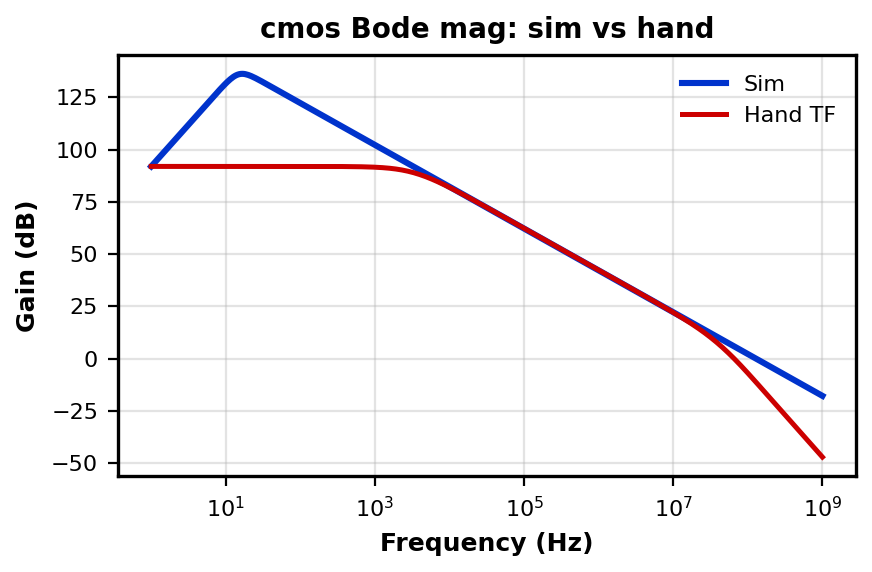
\includegraphics[width=0.88\linewidth]{cmos/figures/bode_mag_overlay.png}
\caption{cmos --- Bode magnitude sim+hand (F1).}\end{figure}
\begin{figure}[ht]\centering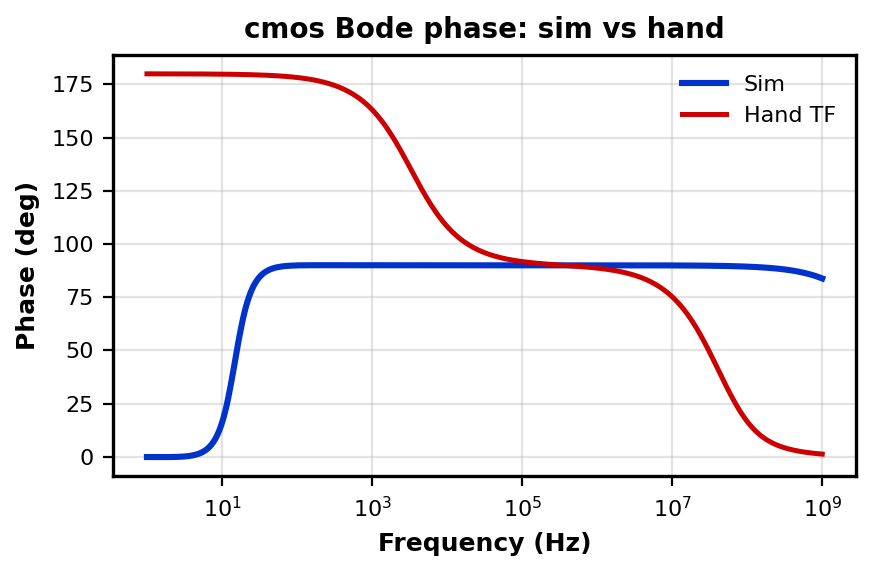
\includegraphics[width=0.88\linewidth]{cmos/figures/bode_phase_overlay.png}
\caption{cmos --- Bode phase sim+hand (F2).}\end{figure}
\begin{figure}[ht]\centering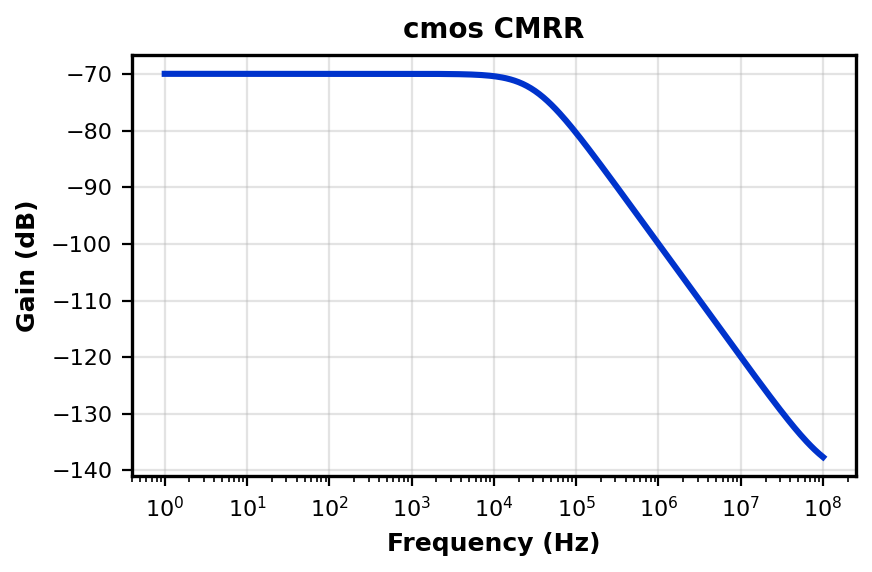
\includegraphics[width=0.88\linewidth]{cmos/figures/cmrr.png}
\caption{cmos --- CMRR vs frequency (F3).}\end{figure}
\begin{figure}[ht]\centering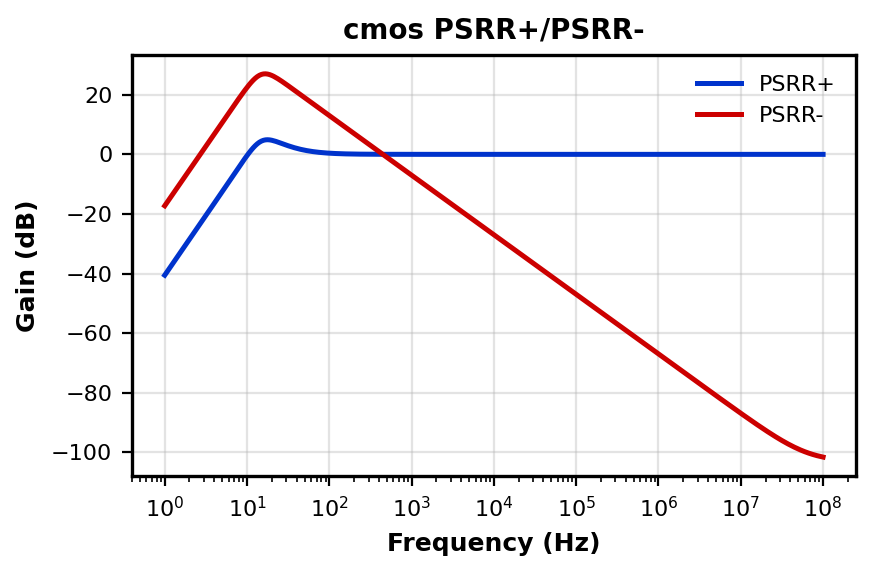
\includegraphics[width=0.88\linewidth]{cmos/figures/psrr.png}
\caption{cmos --- PSRR+ / PSRR- (F4--F5).}\end{figure}
\begin{figure}[ht]\centering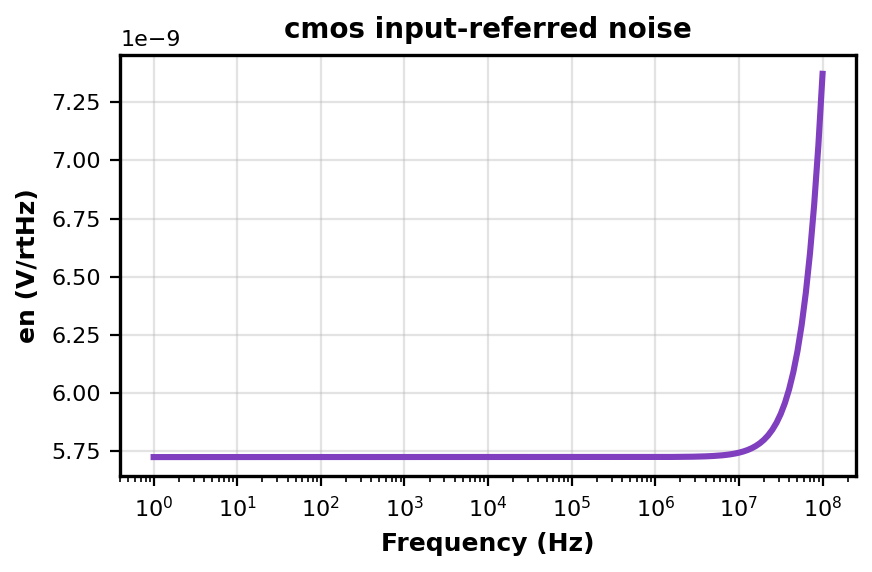
\includegraphics[width=0.88\linewidth]{cmos/figures/noise.png}
\caption{cmos --- input-referred noise density (F6).}\end{figure}
\begin{figure}[ht]\centering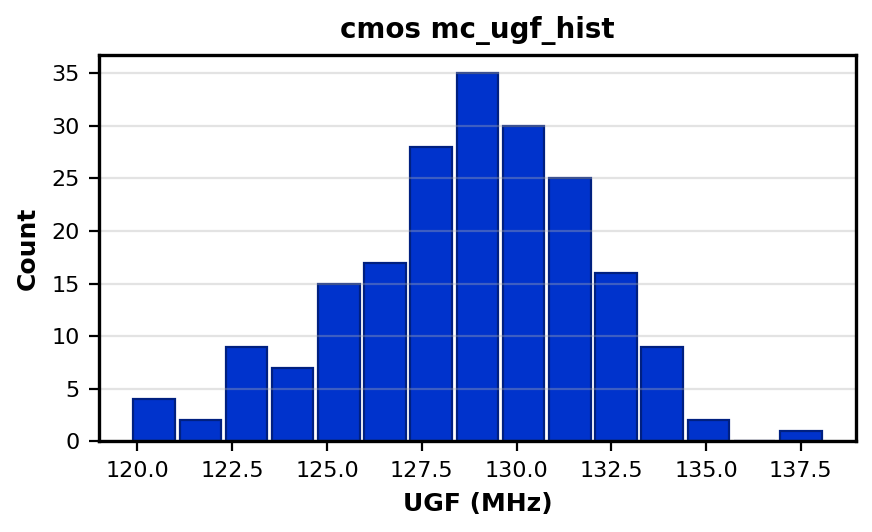
\includegraphics[width=0.88\linewidth]{cmos/figures/mc_ugf_hist.png}
\caption{cmos LOT MC --- UGF histogram (F8), $N=200$.}\end{figure}
\begin{figure}[ht]\centering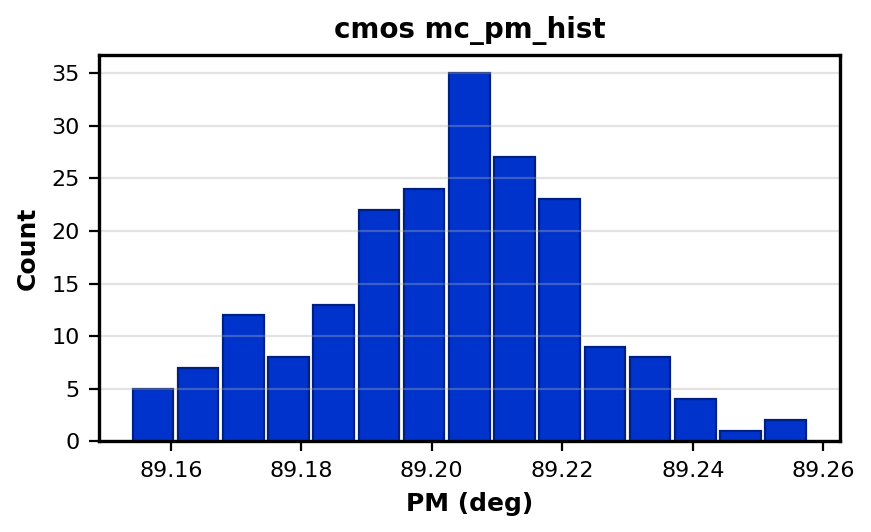
\includegraphics[width=0.88\linewidth]{cmos/figures/mc_pm_hist.png}
\caption{cmos LOT MC --- PM histogram (F9), $N=200$.}\end{figure}
\noindent{\footnotesize Table T8 (cmos): $N=200$, LOT \texttt{mc=1}; UGF mean $128.7\,\mathrm{MHz}$, $\sigma=3.19\,\mathrm{MHz}$; PM mean $89.20^\circ$, $\sigma=0.020^\circ$. Open-PDK MC: HARD-SKIP.}

\section{Results --- sky130}
\subsection{Nominal metrics table}
\begin{center}
{\small\begin{tabular}{@{}lrrrl@{}}
\toprule
Metric & Hand & Sim & Rel.\ error & Match? \\
\midrule
\(A_0\) (dB) & 89.60 & 78.66 & \(+10.94\,\mathrm{dB}\) & FAIL \\
UGF (MHz) & 7.108 & 12.543 & \(-43.3\%\) & FAIL \\
PM (deg) & 72.22 & 81.55 & \(\Delta -9.3^\circ\) & FAIL \\
\(P\) (mW) & 0.963 & 0.963 & \(0\%\) & PASS \\
CMRR (dB) & no hand model & \(-115.5\) & n/a & n/a \\
PSRR+ (dB) & no hand model & \(69.6\) & n/a & n/a \\
PSRR- (dB) & no hand model & \(41.2\) & n/a & n/a \\
\(e_n\) 1\,kHz & no hand model & (2.41 uV/rtHz) & n/a & n/a \\
\(e_n\) 1\,MHz & no hand model & (169.21 nV/rtHz) & n/a & n/a \\
\bottomrule
\end{tabular}}
\end{center}
\footnotesize Table T6 (sky130, primary). Reduced TF under-predicts UGF (starved \(g_{m1}\), parasitics); PM within \(\sim9^\circ\).
\begin{figure}[ht]\centering
\includegraphics[width=0.88\linewidth]{sky130/figures/bode_mag_overlay.png}
\caption{sky130 TT --- Bode magnitude sim+hand (F1).}\end{figure}
\begin{figure}[ht]\centering
\includegraphics[width=0.88\linewidth]{sky130/figures/bode_phase_overlay.png}
\caption{sky130 TT --- Bode phase sim+hand (F2).}\end{figure}
\begin{figure}[ht]\centering
\includegraphics[width=0.88\linewidth]{sky130/figures/cmrr.png}
\caption{sky130 --- CMRR (F3).}\end{figure}
\begin{figure}[ht]\centering
\includegraphics[width=0.88\linewidth]{sky130/figures/psrr.png}
\caption{sky130 --- PSRR (F4--F5).}\end{figure}
\begin{figure}[ht]\centering
\includegraphics[width=0.88\linewidth]{sky130/figures/noise.png}
\caption{sky130 --- noise density (F6).}\end{figure}

\subsection{Corners --- table and figures}
\begin{center}
\begin{tabular}{lrrrr}
\toprule
Corner & \(A_0\) (dB) & UGF (MHz) & PM (deg) & \(P\) (mW) \\
\midrule
tt & 78.66 & 12.543 & 81.55 & 0.963 \\
ff & 82.30 & 51.323 & 102.71 & 0.971 \\
ss & 71.22 & 4.385 & 85.85 & 0.955 \\
\bottomrule
\end{tabular}
\end{center}
\footnotesize Table T7 (sky130).
\begin{figure}[ht]\centering
\includegraphics[width=0.88\linewidth]{sky130/figures/corners_gain.png}
\caption{sky130 corners --- DC gain (F7).}\end{figure}
\begin{figure}[ht]\centering
\includegraphics[width=0.88\linewidth]{sky130/figures/corners_ugf.png}
\caption{sky130 corners --- UGF (F7).}\end{figure}

\subsection{Monte Carlo}
HARD-SKIP: open-PDK mismatch MC not enabled (per-trial agauss slope overrides not wired). Table T8.

\section{Results --- IHP SG13G2}
\begin{center}
{\small\begin{tabular}{@{}lrrrl@{}}
\toprule
Metric & Hand & Sim & Rel.\ error & Match? \\
\midrule
\(A_0\) (dB) & 92.22 & 83.57 & \(+8.65\,\mathrm{dB}\) & FAIL \\
UGF (MHz) & 120.53 & 97.69 & \(+23.4\%\) & FAIL \\
PM (deg) & 3.1 & 97.8 & \(\Delta -94.7^\circ\) & FAIL \\
\(P\) (mW) & 0.628 & 0.628 & \(0\%\) & PASS \\
CMRR (dB) & no hand model & \(-10.8\) & n/a & n/a \\
PSRR+ (dB) & no hand model & \(24.3\) & n/a & n/a \\
PSRR- (dB) & no hand model & \(13.2\) & n/a & n/a \\
\(e_n\) 1\,kHz & no hand model & HARD-SKIP: numerical floor & n/a & n/a \\
\(e_n\) 1\,MHz & no hand model & HARD-SKIP: numerical floor & n/a & n/a \\
\bottomrule
\end{tabular}}
\end{center}
\footnotesize Table T6 (ihp). Hand \(A_0\)/PM/P OP-assisted from sim scalars; GBW from OP \(g_{m1}/(2\pi C_c)\) with \(C_c=1.5\,\mathrm{pF}\), \(g_{m1}=1.136\,\mathrm{mS}\). Noise density numerically tiny (noise TB limitation) --- hard-skip quantitative spots.
\begin{figure}[ht]\centering
\includegraphics[width=0.88\linewidth]{ihp/figures/bode_mag_overlay.png}
\caption{ihp --- Bode magnitude sim+hand (F1).}\end{figure}
\begin{figure}[ht]\centering
\includegraphics[width=0.88\linewidth]{ihp/figures/bode_phase_overlay.png}
\caption{ihp --- Bode phase sim+hand (F2).}\end{figure}
\begin{figure}[ht]\centering
\includegraphics[width=0.88\linewidth]{ihp/figures/cmrr.png}
\caption{ihp --- CMRR (F3).}\end{figure}
\begin{figure}[ht]\centering
\includegraphics[width=0.88\linewidth]{ihp/figures/psrr.png}
\caption{ihp --- PSRR (F4--F5).}\end{figure}
\begin{center}
\begin{tabular}{lrrrr}
\toprule Corner & \(A_0\) & UGF (MHz) & PM & \(P\) (mW) \\
\midrule
tt & 83.57 & 97.69 & 97.83 & 0.628 \\
ff & 83.41 & 98.59 & 99.06 & 0.640 \\
ss & 82.88 & 96.94 & 97.40 & 0.616 \\
\bottomrule
\end{tabular}
\end{center}
\footnotesize Table T7 (ihp).
\begin{figure}[ht]\centering
\includegraphics[width=0.88\linewidth]{ihp/figures/corners_gain.png}
\caption{ihp corners --- gain (F7).}\end{figure}
\begin{figure}[ht]\centering
\includegraphics[width=0.88\linewidth]{ihp/figures/corners_ugf.png}
\caption{ihp corners --- UGF (F7).}\end{figure}
MC: HARD-SKIP (T8).

\section{Results --- GF180}
\begin{center}
{\small\begin{tabular}{@{}lrrrl@{}}
\toprule
Metric & Hand & Sim & Rel.\ error & Match? \\
\midrule
\(A_0\) (dB) & 117.17 & 74.74 & \(+42.43\,\mathrm{dB}\) & FAIL \\
UGF (MHz) & 14.67 & 3.211 & \(+356.9\%\) & FAIL \\
PM (deg) & 36.8 & 89.3 & \(\Delta -52.6^\circ\) & FAIL \\
\(P\) (mW) & 1.441 & 1.441 & \(0\%\) & PASS \\
CMRR (dB) & no hand model & \(-120.1\) & n/a & n/a \\
PSRR+ (dB) & no hand model & \(22.9\) & n/a & n/a \\
PSRR- (dB) & no hand model & \(26.5\) & n/a & n/a \\
\(e_n\) 1\,kHz & no hand model & (3.06 uV/rtHz) & n/a & n/a \\
\(e_n\) 1\,MHz & no hand model & (130.34 nV/rtHz) & n/a & n/a \\
\bottomrule
\end{tabular}}
\end{center}
\footnotesize Table T6 (gf180). Hand GBW \(g_{m1}/(2\pi C_c)\) with \(C_c=2\,\mathrm{pF}\) over-predicts sim UGF (extra poles / loading).
\begin{figure}[ht]\centering
\includegraphics[width=0.88\linewidth]{gf180/figures/bode_mag_overlay.png}
\caption{gf180 --- Bode magnitude sim+hand (F1).}\end{figure}
\begin{figure}[ht]\centering
\includegraphics[width=0.88\linewidth]{gf180/figures/bode_phase_overlay.png}
\caption{gf180 --- Bode phase sim+hand (F2).}\end{figure}
\begin{figure}[ht]\centering
\includegraphics[width=0.88\linewidth]{gf180/figures/cmrr.png}
\caption{gf180 --- CMRR (F3).}\end{figure}
\begin{figure}[ht]\centering
\includegraphics[width=0.88\linewidth]{gf180/figures/psrr.png}
\caption{gf180 --- PSRR (F4--F5).}\end{figure}
\begin{figure}[ht]\centering
\includegraphics[width=0.88\linewidth]{gf180/figures/noise.png}
\caption{gf180 --- noise (F6).}\end{figure}
\begin{center}
\begin{tabular}{lrrrr}
\toprule Corner & \(A_0\) & UGF (MHz) & PM & \(P\) (mW) \\
\midrule
tt & 74.74 & 3.211 & 89.34 & 1.441 \\
ff & 73.55 & 3.287 & 89.34 & 1.460 \\
ss & 75.14 & 3.088 & 89.34 & 1.420 \\
\bottomrule
\end{tabular}
\end{center}
\footnotesize Table T7 (gf180). MC HARD-SKIP (T8).

\section{Cross-backend comparison}
\begin{center}
\begin{tabular}{lrrrr}
\toprule
Backend & \(A_0\) (dB) & UGF (MHz) & PM (deg) & \(P\) (mW) \\
\midrule
cmos & 91.93 & 128.72 & 89.2 & 0.846 \\
sky130 & 78.66 & 12.54 & 81.5 & 0.963 \\
ihp & 83.57 & 97.69 & 97.8 & 0.628 \\
gf180 & 74.74 & 3.21 & 89.3 & 1.441 \\
\bottomrule
\end{tabular}
\end{center}
\footnotesize Table T9.
\begin{figure}[ht]\centering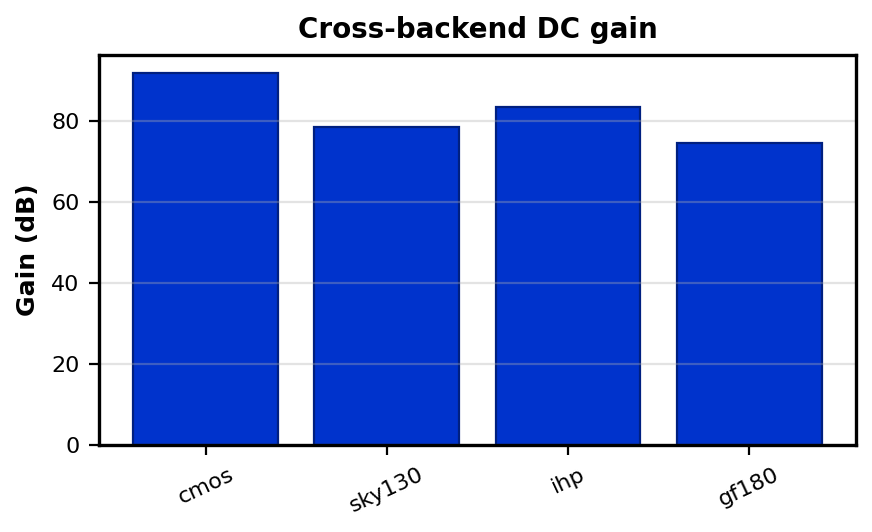
\includegraphics[width=0.88\linewidth]{figures/cross_gain.png}
\caption{Cross-backend DC gain (F10).}\end{figure}
\begin{figure}[ht]\centering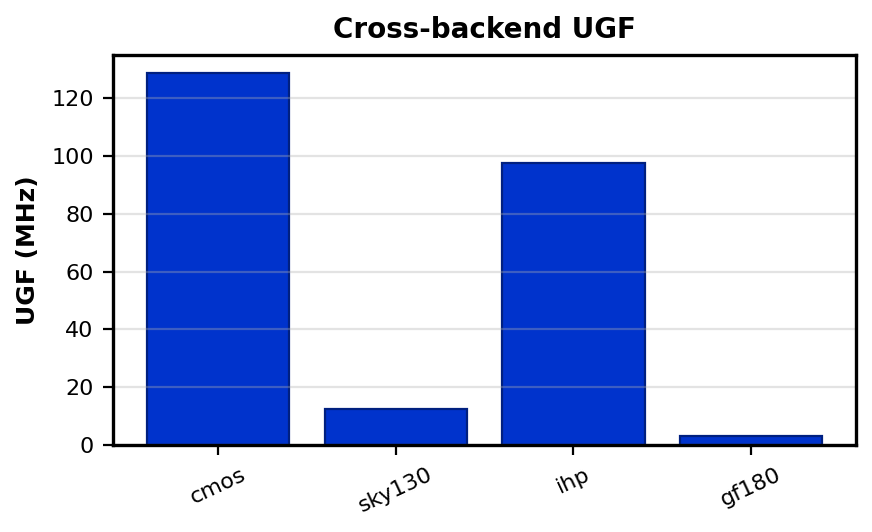
\includegraphics[width=0.88\linewidth]{figures/cross_ugf.png}
\caption{Cross-backend UGF (F10).}\end{figure}
\begin{figure}[ht]\centering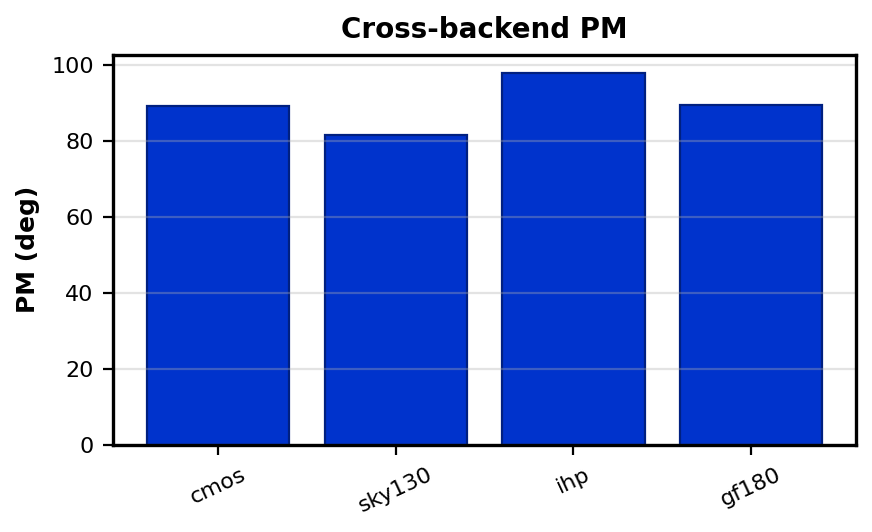
\includegraphics[width=0.88\linewidth]{figures/cross_pm.png}
\caption{Cross-backend PM (F10).}\end{figure}
\begin{figure}[ht]\centering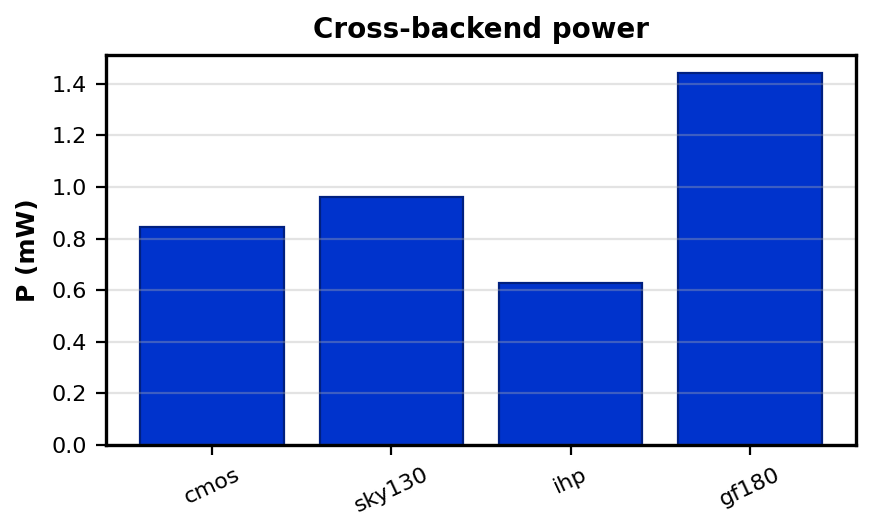
\includegraphics[width=0.88\linewidth]{figures/cross_power.png}
\caption{Cross-backend power (F10).}\end{figure}

\section{Match assessment}
Primary PDK: \textbf{sky130}. Gates: gain \(\pm1\,\mathrm{dB}\), GBW \(\pm5\%\), PM \(\pm5^\circ\), power \(\pm5\%\).
\begin{center}
{\small\begin{tabular}{@{}lrrrl@{}}
\toprule
Metric & Hand & Sim & Tol & Pass? \\
\midrule
\(A_0\) (dB) & 89.60 & 78.66 & \(\pm1\,\mathrm{dB}\) & FAIL \\
UGF (MHz) & 7.108 & 12.543 & \(\pm5\%\) & FAIL \\
PM (deg) & 72.22 & 81.55 & \(\pm5^\circ\) & FAIL \\
\(P\) (mW) & 0.963 & 0.963 & \(\pm5\%\) & PASS \\
\bottomrule
\end{tabular}}
\end{center}
\footnotesize Table T10. FAIL on gain/GBW/PM is expected for reduced 3p1z vs BSIM with starved \(g_{m1}\) and compressed cascode \(g_{ds}\).

\section{Appendix}
\subsection{Notes}
Recovery (sky130): from placeholder \(W=L=1\,\mu\mathrm{m}\) to fitted widths, \(I_b=50\,\mu\mathrm{A}\), \(C_c=1\,\mathrm{pF}\) (see \texttt{sky130/sim} / params).
IHP required \texttt{osdi} (not \texttt{pre\_osdi}) in \texttt{.spiceinit}.
GF180 required \texttt{fnoicor=0} and \texttt{sw\_stat\_*=0}.
MC HARD-SKIP documented above.

\subsection{DUT netlist}
\lstinputlisting{dut_source.sp}
\subsection{Fitted parameters (sky130)}
\lstinputlisting{sky130/tb/params.sp}

\end{document}
